\subsection{Fase 1}

L'equivalente in acqua del calorimetro è pari a:
\begin{equation}
	M_e = (100.0\pm 1.4)\ g
\end{equation}
L'incertezza assoluta è stata ottenuta considerando la stessa incertezza percentuale misurata sul valore stimato della scorsa esperienza. 

La quantità d'acqua versata nel calorimetro è pari a:
\begin{equation}
	M = (200.00\pm 0.01)\ g
\end{equation}

\subsection{Fase 2}

Utilizzando il voltmetro e l'amperometro sono stati misurati i seguenti valori di tensione e corrente:
\begin{equation}
	\Delta V = (5.20\pm 0.01)\ V
\end{equation}

\begin{equation}
	I = (2.46\pm 0.01)\ A
\end{equation}
Non disponendo del manuale di questi strumenti non è stato possibile valutare la reale incertezza di misura. Pertanto, l'incertezza considerata è quella di risoluzione. A questo punto, ogni $60\ s$ è stata misurata la temperatura dell'acqua contenuta nel calorimetro, avendo cura di mescolarla di tanto in tanto.


\begin{table}[H]
	\centering
	\begin{tabular}{|c|c|}
		\hline
		\textbf{Tempo trascorso ($s$)} & \textbf{Temperatura misurata ($^{\circ}C$)} \\
		\hline
		$0$ & $20.3\pm 0.1$ \\
		\hline
		$60.00\pm 0.01$ & $21.0\pm 0.1$ \\
		\hline
		$120.00\pm 0.01$ & $22.3\pm 0.1$ \\
		\hline
		$180.00\pm 0.01$ & $23.4\pm 0.1$ \\
		\hline
		$240.00\pm 0.01$ & $24.2\pm 0.1$ \\
		\hline
		$300.00\pm 0.01$ & $26.1\pm 0.1$ \\
		\hline
		$360.00\pm 0.01$ & $26.6\pm 0.1$ \\
		\hline
		$420.00\pm 0.01$ & $26.1\pm 0.1$ \\
		\hline
		$480.00\pm 0.01$ & $26.6\pm 0.1$ \\
		\hline
		$540.00\pm 0.01$ & $27.1\pm 0.1$ \\
		\hline
		$300.00\pm 0.01$ & $28.9\pm 0.1$ \\
		\hline
	\end{tabular}
	\caption{Qui sono riportate le temperature in corrispondenza del tempo trascorso. A $t=0s$ è associata la temperatura ambiente misurata prima di accendere il generatore di tensione continua.}
	\label{tab:}
\end{table}

A questo punto, tenendo conto che:                    
\begin{equation}
	Q=C_a(M+M_e)\Delta T = C_a(M+M_e)(T-T_0)
\end{equation}
dove $C_a=1 \frac{cal}{g^{\circ}C}$ è il calore specifico dell'acqua e:
\begin{equation}
	E=\Delta VI\Delta t
\end{equation} 

è possibile calcolare i valori di $Q$ ed $E$. Mentre le loro incertezze, tenendo conto della Legge (16), corrispondono a:
\begin{equation}
	\Delta Q = (M_e(T-T_0))\Delta M+(M(T-T0))\Delta M_e+((M+M_e)T_0)\Delta T+((M+M_e)T)\Delta T_0
\end{equation}
\begin{equation}
	\Delta E = (I\Delta t)\delta \Delta V+(\Delta V \Delta t)\Delta I+(\Delta VI)\delta \Delta t
\end{equation}

\begin{figure}[H]
	\centering
	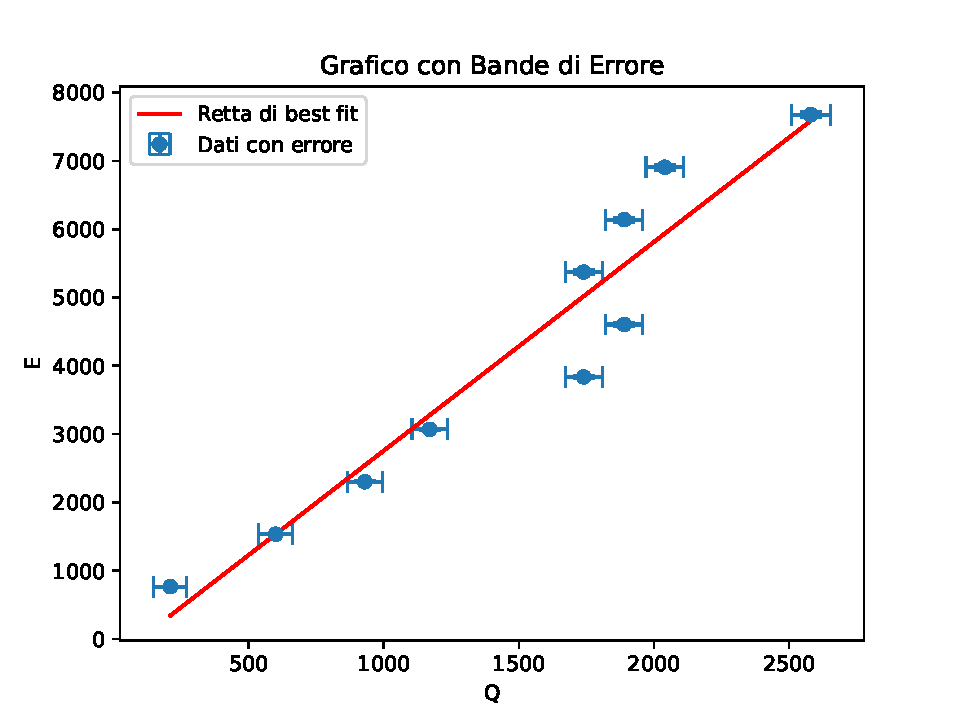
\includegraphics[width=0.99\textwidth]{./figures/grafico1}
	\caption{$E$ in funzione di $Q$.}
\end{figure}
